\documentclass[aspectratio=169]{beamer}

\usetheme{default}
\setbeamertemplate{navigation symbols}{}
\setbeamertemplate{itemize item}{\color{black}\textbullet}
\setbeamertemplate{itemize subitem}{\color{black}\textbullet}
\usepackage{xcolor}
\definecolor{navy}{RGB}{0, 0, 128}

\begin{document}


\begin{frame}

\only<1>{
\begin{align*}
    U_{ij} &= u_{ij} + \underbrace{\epsilon_{ij}}_{\eta_i + \nu_{ij}}\\
    &\\
    &\phantom{= X_i\bar{\beta}_j + Z_j\bar{\gamma} + \underbrace{\epsilon_{ij}}_{\eta_i + \nu_{ij}}}\\
    &\\
    &\phantom{= X_i\bar{\beta}_j + Z_j(\bar{\gamma} + \delta_i) + \nu_{ij}} &\phantom{Z_j\delta_i \equiv \eta_i}\\
    &\\
    &\phantom{= X_i\bar{\beta}_{ij} + Z_j\gamma_{ij} + \nu_{ij}} &\phantom{\beta_{ij}\sim N\left(\bar{\beta},\sigma_\beta^2\right) \gamma_{ij}\sim N\left(\bar{\gamma},\sigma_\gamma^2\right)}
\end{align*}
}

\only<2>{
\begin{align*}
    U_{ij} &= u_{ij} + \underbrace{\epsilon_{ij}}_{\eta_i + \nu_{ij}}\\
    &\\
    &= X_i\bar{\beta}_j + Z_j\bar{\gamma} + \underbrace{\epsilon_{ij}}_{\eta_i + \nu_{ij}}\\
    &\\
    &\phantom{= X_i\bar{\beta}_j + Z_j(\bar{\gamma} + \delta_i) + \nu_{ij}} &\phantom{Z_j\delta_i \equiv \eta_i}\\
    &\\
    &\phantom{= X_i\bar{\beta}_{ij} + Z_j\gamma_{ij} + \nu_{ij}} &\phantom{\beta_{ij}\sim N\left(\bar{\beta},\sigma_\beta^2\right) \gamma_{ij}\sim N\left(\bar{\gamma},\sigma_\gamma^2\right)}
\end{align*}
}

\only<3>{
\begin{align*}
    U_{ij} &= u_{ij} + \underbrace{\epsilon_{ij}}_{\eta_i + \nu_{ij}}\\
    &\\
    &= X_i\bar{\beta}_j + Z_j\bar{\gamma} + \underbrace{\epsilon_{ij}}_{\eta_i + \nu_{ij}}\\
    &\\
    &= X_i\left(\bar{\beta}_j + \delta_i\right) + Z_j\left(\bar{\gamma} + \phi_i\right) + \nu_{ij}& X_i\delta_i + Z_j\phi_i \equiv \eta_i\\
    &\\
    &\phantom{= X_i\bar{\beta}_{ij} + Z_j\gamma_{i} + \nu_{ij}} &\phantom{\beta_{ij}\sim N\left(\bar{\beta}_j,\sigma_\beta^2\right) \gamma_{i}\sim N\left(\bar{\gamma},\sigma_\gamma^2\right)}
\end{align*}
}

\only<4>{
\begin{align*}
    U_{ij} &= u_{ij} + \underbrace{\epsilon_{ij}}_{\eta_i + \nu_{ij}}\\
    &\\
    &= X_i\bar{\beta}_j + Z_j\bar{\gamma} + \underbrace{\epsilon_{ij}}_{\eta_i + \nu_{ij}}\\
    &\\
    &= X_i\left(\bar{\beta}_j + \delta_i\right) + Z_j\left(\bar{\gamma} + \phi_i\right) + \nu_{ij}&  X_i\delta_i + Z_j\phi_i \equiv \eta_i\\
    &\\
    &= X_i\beta_{ij} + Z_j\gamma_{i} + \nu_{ij} &\beta_{ij}\sim N\left(\bar{\beta}_j,\sigma_\beta^2\right),\,\, \gamma_{i}\sim N\left(\bar{\gamma},\sigma_\gamma^2\right)
\end{align*}
}

\end{frame}


\begin{frame}

Parametric identification: assume mixing distribution shape, estimate parameters

\bigskip

\onslide<2->{
But this just pushes problem back one level...
}

\bigskip

\onslide<3->{
How can we know if choice variation comes from $\eta_i$ or $\nu_{ij}$ part of preferences?
}

\end{frame}

\begin{frame}

Cross-sectional data: impossible to separate

\bigskip

Person A chooses different alternative than Person B
\bigskip

\onslide<2->{
$\Rightarrow$ Different tastes? Or different random shocks?
}

\bigskip

\onslide<3->{
Single observation per person provides no way to distinguish
}

\end{frame}

\begin{frame}

Panel data solution: same person, multiple choice situations

\bigskip

\onslide<2->{
Persistent patterns across periods $\Rightarrow$ permanent tastes ($\delta_i,\phi_i$)
}

\bigskip

\onslide<3->{
Random variation across periods $\Rightarrow$ idiosyncratic tastes ($\epsilon_{ijt}$)
}

\bigskip

\onslide<4->{
Key assumption: tastes $\delta_i,\phi_i$ stable across choice instances for each person
}

\end{frame}

\begin{frame}

Identification logic:

\bigskip

Person consistently chooses similar alternatives across $T$ situations
\bigskip

\onslide<2->{
$\Rightarrow$ Reveals their $\delta_i,\phi_i$ (permanent taste parameters)
}

\bigskip

\onslide<3->{
Larger $T \rightarrow$ better separation of $\delta_i,\phi_i$ from noise
}

\bigskip

\onslide<4->{
$T \rightarrow \infty \Rightarrow$ can perfectly identify each person's $\delta_i,\phi_i$
}

\end{frame}




\begin{frame}

\only<1-3,5->{
Different types of variation can identify taste heterogeneity:

\bigskip

}

\only<2-3,5->{
Panel data: Same person, multiple choice situations

\bigskip

}

\only<3,5->{
Persistent choices across time $\Rightarrow$ reveals individual $\delta_i,\phi_i$

\bigskip

}

\only<4>{
\begin{center}
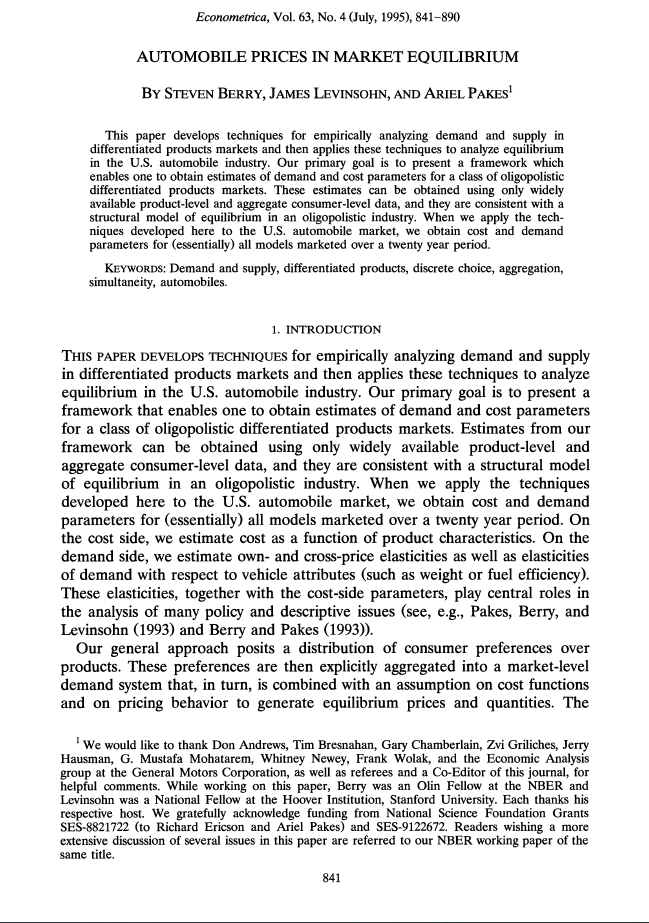
\includegraphics[width=0.4\textwidth]{blp_cover.jpg}
\end{center}
}

\only<5->{
Berry, Levinsohn, Pakes (1995) approach: Multiple markets, aggregate shares

\bigskip

}

\only<6->{
Substitution patterns across products within markets $\Rightarrow$ reveals distribution of $\delta_i,\phi_i$

\bigskip

}

\only<7->{
Alternative: Use exclusion restrictions/valid instruments when panel data unavailable

\bigskip

}

\only<8->{
Key insight: Many ways of leveraging variation to separate $\delta_i,\phi_i$ from $\nu_{ij}$
}

\end{frame}


\end{document}